\chapter{Comment surveiller un musée}\label{c.museum}

%%%%%%%%%%%%%%%%%%%%%%%%%%%%%%%%%%%%%%%%%%%%%%%%%%%%%%%%%%%%%%%



%%%%%%%%%%%%%%%%%%%%%%%%%%%%%%%%%%%%%%%%%%%%%%%%%%%%%%%%%%%%%%%

En 1973, Victor Klee s'est demandé combien de gardiens sont nécessaires pour surveiller tous les murs d'un musée ? Si les murs forment un polygone régulier ou même un polygone convexe, un gardien suffit (fig.~\ref{f.museum.convex}).

\begin{figure}[htbp]
\centering
\begin{tikzpicture}[scale=.6]
\coordinate (O) at (0,0);
\vertex{O};
\foreach \x/\name/\n/\po in {0/a/A/right,.6/b/B/above,1.6/c/C/left,2.4/d/D/below left,3.9/e/E/below right} {
  \coordinate (\name) at ($(O)+(\x*72+18:3cm)$);
\draw[dashed] (O) -- (\name);
}
\draw (a) -- (b) -- (c) -- (d) --(e) -- cycle;
\end{tikzpicture}
%\includegraphics[width=0.5\textwidth]{Fig5_1}
\caption{Un musée dont les murs forment un polygone convexe.}\label{f.museum.convex}
\end{figure}

Considérons maintenant un musée dont les murs sont en dents de scie (fig.~\ref{f.museum.nonconvex}). On vérifie en comptant que le musée a 15 murs. Chaque \og dent\fg{} définit un triangle qui est grisé  dans la figure~\ref{f.visibility-tooth}. Un gardien placé n'importe où dans l'un des triangles peut observer tous les murs qui délimitent ce triangle (flèches rouges).

\begin{figure}[htbp]
\centering
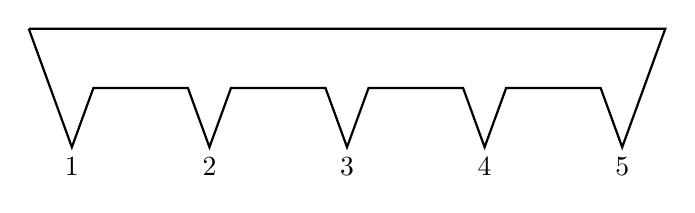
\begin{tikzpicture}[scale=.8]
\coordinate (O) at (0,0);
\draw [thick] (O) -- (++110:1cm) coordinate (P);
\draw[thick] (O) --
  ++(-70:1cm) coordinate(A) node[below] {$1$} -- 
  ++(+70:1cm) -- ++(0:1.5cm) --
  ++(-70:1cm) coordinate(B) node[below] {$2$} -- 
  ++(+70:1cm) -- ++(0:1.5cm) --
  ++(-70:1cm) coordinate(C) node[below] {$3$}-- 
  ++(+70:1cm) -- ++(0:1.5cm) --
  ++(-70:1cm) coordinate(D) node[below] {$4$} -- 
  ++(+70:1cm) -- ++(0:1.5cm) --
  ++(-70:1cm) coordinate(E) node[below] {$5$} --
  ++(+70:2cm) -- (P);

\end{tikzpicture}
%\includegraphics[width=0.5\textwidth]{Fig5_2}
\caption{Un musée dont les murs ne forment pas un polygone convexe.}
\label{f.museum.nonconvex}
\end{figure}

\begin{figure}[htbp]
\centering
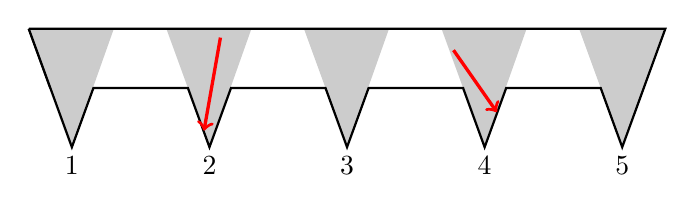
\begin{tikzpicture}[scale=.8]
\coordinate (O) at (0,0);
\draw [thick] (O) -- (++110:1cm) coordinate (P);
\path (O) --
  ++(-70:1cm) coordinate(A) node[below] {$1$} -- 
  ++(+70:1cm) coordinate(A1) -- ++(0:1.5cm) coordinate(A2) --
  ++(-70:1cm) coordinate(B) node[below] {$2$} -- 
  ++(+70:1cm) coordinate(B1) -- ++(0:1.5cm) coordinate(B2) --
  ++(-70:1cm) coordinate(C) node[below] {$3$}-- 
  ++(+70:1cm) coordinate(C1) -- ++(0:1.5cm) coordinate(C2) --
  ++(-70:1cm) coordinate(D) node[below] {$4$} -- 
  ++(+70:1cm) coordinate(D1) -- ++(0:1.5cm) coordinate(D2) --
  ++(-70:1cm) coordinate(E) node[below] {$5$} --
  ++(+70:2cm) coordinate(E1) -- (P);

\path[fill,black!20!white] (A) -- ++(110:2cm) -- ++(0:1.35cm)-- cycle;
\path[fill,black!20!white] (B) -- ++(110:2cm) -- ++(0:1.35cm)-- cycle;
\path[fill,black!20!white] (C) -- ++(110:2cm) -- ++(0:1.35cm)-- cycle;
\path[fill,black!20!white] (D) -- ++(110:2cm) -- ++(0:1.35cm)-- cycle;
\path[fill,black!20!white] (E) -- ++(110:2cm) -- ++(0:1.35cm)-- cycle;

\draw[thick] (P) -- (O) -- (A) -- (A1) -- (A2) --
   (B) -- (B1) -- (B2) -- (C) -- (C1) -- (C2) --
   (D) -- (D1) -- (D2) -- (E) -- (E1) -- (P);

\coordinate (G1) at (2.7,.8);
\coordinate (G2) at (6.4,.6);
\draw[->,red,very thick] (G1) -- +(-100:1.5cm);
\draw[->,red,very thick] (G2) -- +(-55:1.2cm);
\vertexcolor{G1}{red};
\vertexcolor{G2}{red};
\end{tikzpicture}
%\includegraphics[width=0.5\textwidth]{Fig5_3}
\caption{Visibilité à l'intérieur de chaque \og dent\fg.}
\label{f.visibility-tooth}
\end{figure}

Si au moins l'un des gardiens est placé près du mur supérieur couvrant l'ensemble du musée, il peut observer tous les murs horizontaux (flèches bleues dans la figure~\ref{f.museum.shaded}). Ainsi, $5=15/3$ gardiens sont suffisants pour observer tous les murs du musée. Comme les triangles ne se chevauchent pas, le gardien d'un triangle ne pourra pas observer tous les murs d'un autre triangle (flèche verte) ; il faut donc 5 gardiens.

\begin{figure}[htbp]
\centering
\begin{tikzpicture}[scale=.8]
\coordinate (O) at (0,0);
\draw [thick] (O) -- (++110:1cm) coordinate (P);
\path (O) --
  ++(-70:1cm) coordinate(A) node[below] {$1$} -- 
  ++(+70:1cm) coordinate(A1) -- ++(0:1.5cm) coordinate(A2) --
  ++(-70:1cm) coordinate(B) node[below] {$2$} -- 
  ++(+70:1cm) coordinate(B1) -- ++(0:1.5cm) coordinate(B2) --
  ++(-70:1cm) coordinate(C) node[below] {$3$}-- 
  ++(+70:1cm) coordinate(C1) -- ++(0:1.5cm) coordinate(C2) --
  ++(-70:1cm) coordinate(D) node[below] {$4$} -- 
  ++(+70:1cm) coordinate(D1) -- ++(0:1.5cm) coordinate(D2) --
  ++(-70:1cm) coordinate(E) node[below] {$5$} --
  ++(+70:2cm) coordinate(E1) -- (P);

\path[fill,black!20!white] (A) -- ++(110:2cm) -- ++(0:1.35cm)-- cycle;
\path[fill,black!20!white] (B) -- ++(110:2cm) -- ++(0:1.35cm)-- cycle;
\path[fill,black!20!white] (C) -- ++(110:2cm) -- ++(0:1.35cm)-- cycle;
\path[fill,black!20!white] (D) -- ++(110:2cm) -- ++(0:1.35cm)-- cycle;
\path[fill,black!20!white] (E) -- ++(110:2cm) -- ++(0:1.35cm)-- cycle;

\draw[thick] (P) -- (O) -- (A) -- (A1) -- (A2) --
   (B) -- (B1) -- (B2) -- (C) -- (C1) -- (C2) --
   (D) -- (D1) -- (D2) -- (E) -- (E1) -- (P);

\coordinate (G1) at (9,.8);
\coordinate (G2) at ($(O)+(.5,.5)$);
\draw[->,very thick,green!80!black,dashed] (G1) -- +(-165:4.6cm);
\draw[->,very thick,blue] (G2) -- ++(7.4,.35);
\draw[->,very thick,blue] (G2) -- ++(2.9,-.42);
\draw[thick] (6,0) circle(4pt);
\draw[thick] (4.95,-.28) circle(4pt);
\vertexcolor{G1}{green!80!black};
\vertexcolor{G2}{blue};
\end{tikzpicture}
%\includegraphics[width=0.5\textwidth]{Fig5_4}
\caption{Visibilité des murs du musée.}\label{f.museum.shaded}
\end{figure}

L'exemple de la figure~\ref{f.museum.nonconvex} peut être généralisé à $n/3$ dents avec $n$ murs, nous concluons donc qu'au moins $n/3$ gardiens sont nécessaires. Nous souhaitons démontrer que $n/3$ gardiens sont suffisants pour surveiller un musée quelconque.

La section~\ref{s.museum-triangulating} démontre que tout polygone triangulé peut être colorié avec trois couleurs. Ceci est utilisé dans la section~\ref{s.museum-guard} pour démontrer le théorème selon lequel $n/3$ gardiens sont suffisants. La section~\ref{s.museum-triangulated} complète la démonstration en montrant que tout polygone peut être triangulé.

\section{Coloration des polygones triangulés}\label{s.museum-triangulating}

\begin{definition}
Une \emph{diagonale} d'un polygone est une arête reliant deux sommets qui n'est pas une des arêtes (extérieures) du polygone.
\end{definition}

\begin{definition} Un polygone peut être \emph{triangulé} si l'on peut construire des diagonales qui ne s'entrecoupent pas de telle sorte que l'intérieur du polygone soit recouvert de triangles.
\end{definition}
\vspace{-2ex}
\begin{theorem}
Tout polygone peut être triangulé.\label{thm.tri}
\end{theorem}
Nous différons la démonstration du théorème~\ref{thm.tri}.
\begin{definition}
Un sommet d'un polygone est \emph{convexe} si son angle intérieur est inférieur à $180^\circ$ ; un sommet est \emph{concave} si son angle intérieur est supérieur à $180^\circ$. 
\end{definition}
Dans la  figure~\ref{f.museum.arbitrary}, le sommet $1$ est convexe et le sommet $2$ est concave.

\begin{figure}[htbp]
\centering
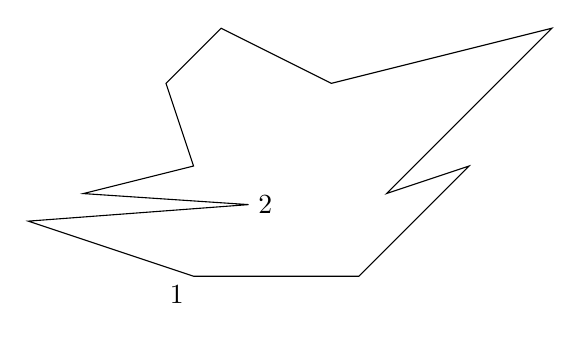
\begin{tikzpicture}[scale=.7]
\draw
  (0,0) coordinate (A) node[below left] {$1$} -- 
  ++(3,0) coordinate (B) --
  ++(2,2) coordinate (C) --
  ++(-1.5,-.5) coordinate (D) --
  ++(3,3) coordinate (E) -- 
  ++(-4,-1) coordinate (F) --
  ++(-2,1) coordinate (G) --
  ++(-1,-1) coordinate (H) --
  ++(.5,-1.5) coordinate (I) --
  ++(-2,-.5) coordinate (J) --
  ++(3,-.2) coordinate (K) node[right] {$2$} -- 
  ++(-4,-.3) coordinate (L) --
  cycle;
\vertex{A};
\vertex{K};
\end{tikzpicture}
%\includegraphics[width=0.5\textwidth]{Fig5_5}
\caption{Un polygone avec un sommet convexe ($1$) et un sommet concave~($2$).}
\label{f.museum.arbitrary}
\end{figure}

\begin{definition}
Un polygone avec des sommets $V$ peut être \emph{colorié avec trois couleurs} s'il existe une application 
\[c: V \mapsto \{\mathit{rouge},\mathit{bleu},\mathit{vert}\}\,\] 
telle qu'aucune arête n'ait deux sommets qui ont la même couleur.
\end{definition}

\begin{theorem}
Un polygone triangulé peut être colorié avec trois couleurs.\label{thm.colored}
\end{theorem}

\begin{proof}
Par récurrence sur le nombre de sommets. Un triangle peut être colorié avec trois couleurs. Un polygone triangulé avec $n>3$ sommets doit avoir une diagonale. Choisissons une diagonale arbitraire $\overline{AB}$ (fig.~\ref{f.museum.three-1}) et divisons le polygone le long de cette diagonale en deux polygones plus petits (fig.~\ref{f.museum.three-2}). Par récurrence, chacun de ces petits polygones peut être colorié avec trois couleurs  (fig.~\ref{f.museum.three-3}).

Puisque les couleurs attribuées sont arbitraires, si des couleurs différentes sont attribuées à $A$ et à $B$ dans les deux polygones, nous pouvons renommer les couleurs dans l'un d'entre eux afin que les couleurs de $A$ et $B$ soient les mêmes dans les deux polygones. Par exemple, dans la figure~\ref{f.museum.three-4}, on peut échanger \emph{rouge} et \emph{vert} dans le polygone inférieur.
Collons les deux polygones ensemble pour récupérer le polygone original avec $n$ sommets. Il sera colorié avec trois couleurs  (fig.~\ref{f.museum.three-5}).\qedhere
\end{proof}

\vspace{0.4cm}

\begin{minipage}{0.42\textwidth}
\centering    
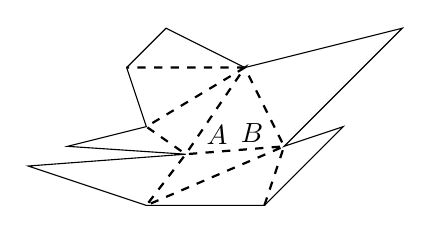
\begin{tikzpicture}[scale=.5]
\draw
  (0,0) coordinate (A) -- 
  ++(3,0) coordinate (B) --
  ++(2,2) coordinate (C) --
  ++(-1.5,-.5) coordinate (D) --
  ++(3,3) coordinate (E) -- 
  ++(-4,-1) coordinate (F) --
  ++(-2,1) coordinate (G) --
  ++(-1,-1) coordinate (H) --
  ++(.5,-1.5) coordinate (I) --
  ++(-2,-.5) coordinate (J) --
  ++(3,-.2) coordinate (K) -- 
  ++(-4,-.3) coordinate (L) --
  cycle;
\vertex{K};
\vertex{D};
\node[above right,xshift=4pt] at (K) {$A$};
\node[above left,xshift=-4pt,yshift=-2pt] at (D) {$B$};

\draw[thick,dashed]
  (B) -- (D) -- (K) -- (F) -- (I) -- (K) -- (A) -- (D) -- (F) -- (H);
\end{tikzpicture}
%\includegraphics[width=\textwidth]{Fig5_6a}
         \captionof{figure}{Une diagonale arbitraire dans un polygone.}
         \label{f.museum.three-1}
     \end{minipage}
     \quad \ %\hspace{3em}
     \begin{minipage}{0.42\textwidth}
\centering      
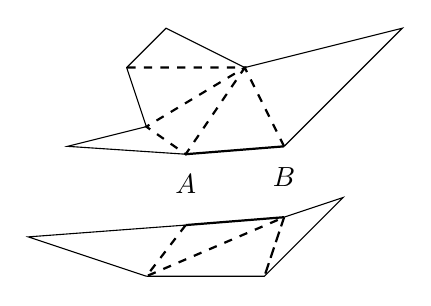
\begin{tikzpicture}[scale=.5]
\path
  (0,0) coordinate (A1) -- 
  ++(3,0) coordinate (B1) --
  ++(2,2) coordinate (C1) --
  ++(-1.5,-.5) coordinate (D1);
\draw
  (D1) --
  ++(3,3) coordinate (E1) -- 
  ++(-4,-1) coordinate (F1) --
  ++(-2,1) coordinate (G1) --
  ++(-1,-1) coordinate (H1) --
  ++(.5,-1.5) coordinate (I1) --
  ++(-2,-.5) coordinate (J1) --
  ++(3,-.2) coordinate (K1);
\path
  (K1) -- 
  ++(-4,-.3) coordinate (L1) --
  (A1);
\vertex{K1};
\vertex{D1};
\node[below,yshift=-4pt] at (K1) {$A$};
\node[below,yshift=-4pt] at (D1) {$B$};

\draw[thick,dashed]
  (D1) -- (F1) -- (I1) -- (K1) -- (F1) -- (H1);
\draw[thick] (D1) -- (K1);


\begin{scope}[yshift=-1.8cm]

\draw
  (0,0) coordinate (A2) -- 
  ++(3,0) coordinate (B2) --
  ++(2,2) coordinate (C2) --
  ++(-1.5,-.5) coordinate (D2);
\path
  (D2) --
  ++(3,3) coordinate (E2) --
  ++(-4,-1) coordinate (F2) --
  ++(-2,1) coordinate (G2) --
  ++(-1,-1) coordinate (H2) --
  ++(.5,-1.5) coordinate (I2) --
  ++(-2,-.5) coordinate (J2) --
  ++(3,-.2) coordinate (K2);
\draw
  (K2) --
  ++(-4,-.3) coordinate (L2) --
  (A2);
\vertex{K2};
\vertex{D2}; 
%\node[above,yshift=4pt] at (K2) {$A$};
%\node[above,yshift=4pt] at (D2) {$B$};

\draw[thick,dashed]
  (K2) -- (A2) -- (D2) -- (B2) -- (D2);
\draw[thick] (D2) -- (K2);

\end{scope}
\end{tikzpicture}
%\includegraphics[width=\textwidth]{Fig5_6b}
         \captionof{figure}
         {Division  du  polygone.}\label{f.museum.three-2}
     \end{minipage}

\vspace{0.4cm}

\begin{minipage}{0.42\textwidth}
\centering     
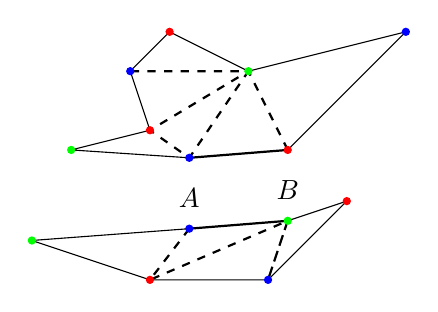
\begin{tikzpicture}[scale=.5]
\path
  (0,0) coordinate (A1) -- 
  ++(3,0) coordinate (B1) --
  ++(2,2) coordinate (C1) --
  ++(-1.5,-.5) coordinate (D1);
\draw
  (D1) --
  ++(3,3) coordinate (E1) -- 
  ++(-4,-1) coordinate (F1) --
  ++(-2,1) coordinate (G1) --
  ++(-1,-1) coordinate (H1) --
  ++(.5,-1.5) coordinate (I1) --
  ++(-2,-.5) coordinate (J1) --
  ++(3,-.2) coordinate (K1);
\path
  (K1) -- 
  ++(-4,-.3) coordinate (L1) --
  (A1);
  
\draw[thick,dashed]
  (D1) -- (F1) -- (I1) -- (K1) -- (F1) -- (H1);
\draw[thick] (D1) -- (K1);

%\node[below,yshift=-4pt] at (K1) {$A$};
%\node[below,yshift=-4pt] at (D1) {$B$};

\foreach \point/\color in {D1/red,E1/blue,F1/green,G1/red,H1/blue,I1/red,J1/green,K1/blue}
  \fill[color=\color] (\point) circle(3pt);

\begin{scope}[yshift=-1.8cm]

\draw
  (0,0) coordinate (A2) -- 
  ++(3,0) coordinate (B2) --
  ++(2,2) coordinate (C2) --
  ++(-1.5,-.5) coordinate (D2);
\path
  (D2) --
  ++(3,3) coordinate (E2) --
  ++(-4,-1) coordinate (F2) --
  ++(-2,1) coordinate (G2) --
  ++(-1,-1) coordinate (H2) --
  ++(.5,-1.5) coordinate (I2) --
  ++(-2,-.5) coordinate (J2) --
  ++(3,-.2) coordinate (K2);
\draw
  (K2) --
  ++(-4,-.3) coordinate (L2) --
  (A2);
  
\draw[thick,dashed]
  (K2) -- (A2) -- (D2) -- (B2) -- (D2);
\draw[thick] (D2) -- (K2);
\node[above,yshift=4pt] at (K2) {$A$};
\node[above,yshift=4pt] at (D2) {$B$};

\foreach \point/\color in {A2/red,B2/blue,C2/red,D2/green,K2/blue,L2/green}
  \fill[color=\color] (\point) circle(3pt);

\end{scope}
\end{tikzpicture}
%\includegraphics[width=\textwidth]{Fig5_7a}
         \captionof{figure}{Coloriage des deux plus petits polygones.}
\label{f.museum.three-3}
\end{minipage}
\quad \ %\hspace{3em}
    \begin{minipage}{0.42\textwidth}
\centering       
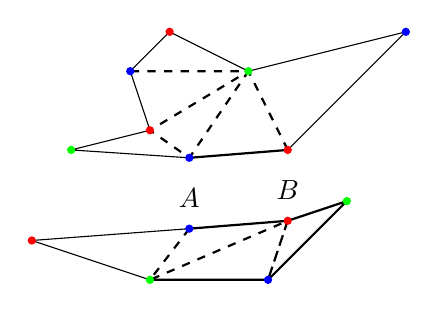
\begin{tikzpicture}[scale=.5]
\path
  (0,0) coordinate (A1) -- 
  ++(3,0) coordinate (B1) --
  ++(2,2) coordinate (C1) --
  ++(-1.5,-.5) coordinate (D1);
\draw
  (D1) --
  ++(3,3) coordinate (E1) -- 
  ++(-4,-1) coordinate (F1) --
  ++(-2,1) coordinate (G1) --
  ++(-1,-1) coordinate (H1) --
  ++(.5,-1.5) coordinate (I1) --
  ++(-2,-.5) coordinate (J1) --
  ++(3,-.2) coordinate (K1);
\path
  (K1) -- 
  ++(-4,-.3) coordinate (L1) --
  (A1);
  
%\node[below,yshift=-4pt] at (K1) {$A$};
%\node[below,yshift=-4pt] at (D1) {$B$};

\draw[thick,dashed]
  (D1) -- (F1) -- (I1) -- (K1) -- (F1) -- (H1);
\draw[thick] (D1) -- (K1);

\foreach \point/\color in {D1/red,E1/blue,F1/green,G1/red,H1/blue,I1/red,J1/green,K1/blue}
  \fill[color=\color] (\point) circle(3pt);

\begin{scope}[yshift=-1.8cm]

\draw[thick]
  (0,0) coordinate (A2) -- 
  ++(3,0) coordinate (B2) --
  ++(2,2) coordinate (C2) --
  ++(-1.5,-.5) coordinate (D2);
\path
  (D2) --
  ++(3,3) coordinate (E2) --
  ++(-4,-1) coordinate (F2) --
  ++(-2,1) coordinate (G2) --
  ++(-1,-1) coordinate (H2) --
  ++(.5,-1.5) coordinate (I2) --
  ++(-2,-.5) coordinate (J2) --
  ++(3,-.2) coordinate (K2);
\draw
  (K2) --
  ++(-4,-.3) coordinate (L2) --
  (A2);
  
\draw[thick,dashed]
  (K2) -- (A2) -- (D2) -- (B2) -- (D2);
\draw[thick] (D2) -- (K2);
\node[above,yshift=4pt] at (K2) {$A$};
\node[above,yshift=4pt] at (D2) {$B$};

\foreach \point/\color in {A2/green,B2/blue,C2/green,D2/red,K2/blue,L2/red}
  \fill[color=\color] (\point) circle(3pt);

\end{scope}
\end{tikzpicture}
%\includegraphics[width=\textwidth]{Fig5_7b}
         \captionof{figure}{Échange des couleurs d'un polygone pour qu'elles correspondent à celles de l'autre.}
         \label{f.museum.three-4}
\end{minipage}

\begin{figure}[htbp]
\centering
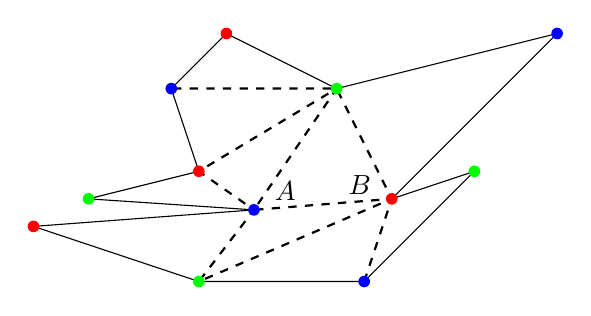
\begin{tikzpicture}[scale=.7]
\draw
  (0,0) coordinate (A) -- 
  ++(3,0) coordinate (B) --
  ++(2,2) coordinate (C) --
  ++(-1.5,-.5) coordinate (D) --
  ++(3,3) coordinate (E) -- 
  ++(-4,-1) coordinate (F) --
  ++(-2,1) coordinate (G) --
  ++(-1,-1) coordinate (H) --
  ++(.5,-1.5) coordinate (I) --
  ++(-2,-.5) coordinate (J) --
  ++(3,-.2) coordinate (K) -- 
  ++(-4,-.3) coordinate (L) --
  cycle;
  
\node[above right,xshift=4pt] at (K) {$A$};
\node[above left,xshift=-4pt,yshift=-2pt] at (D) {$B$};

\draw[thick,dashed]
  (B) -- (D) -- (K) -- (F) -- (I) -- (K) -- (A) -- (D) -- (F) -- (H);

\foreach \point/\color in {D/red,E/blue,F/green,G/red,H/blue,I/red,J/green,K/blue,A/green,B/blue,C/green,L/red}
  \fill[color=\color] (\point) circle(3pt);

\end{tikzpicture}
%\includegraphics[width=0.8\textwidth]{Fig5_8}
\caption{Recollement des deux petits polygones.}
\label{f.museum.three-5}
\end{figure}



\section{Du coloriage de polygones à la surveillance d'un musée}\label{s.museum-guard}

\begin{theorem}\label{thm.guarded} Un musée avec $n$ murs peut être surveillé par $n/3$ gardiens.
\end{theorem}
\begin{proof}
D'après le théorème~\ref{thm.tri},  le polygone peut être triangulé. D'après le théorème~\ref{thm.colored},  le polygone peut être colorié avec trois couleurs. Les trois sommets de chaque triangle de la triangulation doivent être coloriés avec des couleurs différentes afin de satisfaire la condition de trichromie. Puisque le polygone est colorié avec trois couleurs, au moins une couleur, disons le rouge, peut apparaître au plus $n/3$ fois, et chaque triangle doit avoir un sommet colorié en rouge. Postons un gardien à chaque sommet rouge; il peut observer tous les murs de chaque triangle auquel le sommet appartient. Puisque les triangles de la triangulation incluent toutes les arêtes du polygone, $n/3$ gardiens sont suffisants pour surveiller tous les murs du musée.
\end{proof}
Si $n$ n'est pas divisible par $3$, le nombre de gardiens nécessaire est $\lfloor n/3\rfloor$, le plus grand nombre entier inférieur ou égal à $n/3$. Par exemple, 4 gardiens sont suffisants pour les musées à 12, 13 ou 14 murs puisque $\lfloor 12/3\rfloor =\lfloor 13/3\rfloor=\lfloor 14/3\rfloor=4$. Pour simplifier, nous ignorons cette complication.
 
\section{Tout polygone peut être triangulé}\label{s.museum-triangulated}

\begin{theorem}\label{thm.interior-angles-of-a-polygon}
La somme des angles intérieurs d'un polygone à $n$ sommets est 
\[180^\circ(n-2)\,.\]
\end{theorem}
\begin{proof}
Considérons un polygone convexe et désignons ses angles extérieurs par $\theta_i$ (fig.~\ref{f.museum.exterior}).
En passant d'une ligne pointillée à la suivante, on effectue une rotation autour d'un cercle :
\[
\sum_{i=1}^n \theta_i = 360^\circ\,.
\]

\begin{figure}[htbp]
\centering
\begin{tikzpicture}[scale=.5]
\coordinate (O) at (0,0);
\foreach \x/\name/\n/\po in {0/a/A/right,.6/b/B/above,1.6/c/C/left,2.4/d/D/below left,3.9/e/E/below right} {
  \coordinate (\name) at ($(O)+(\x*72+18:3cm)$);
}
\draw[thick] (a) -- (b) -- (c) -- (d) --(e) -- cycle;

\draw[thick,dashed] (a) 
  node[above,xshift=-2pt,yshift=8pt] {$\theta_1$} -- 
  ($(a)!2!(b)$);
\draw[thick,dashed] (b)
  node[above left,xshift=-8pt,yshift=0pt] {$\theta_2$} -- 
  ($(b)!1.7!(c)$);
\draw[thick,dashed] (c) 
  node[below left,xshift=-4pt,yshift=-2pt] {$\theta_3$} -- 
  ($(c)!1.7!(d)$);
\draw[thick,dashed] (d)
  node[below right,xshift=0pt,yshift=-4pt] {$\theta_4$} -- 
  ($(d)!1.5!(e)$);
\draw[thick,dashed] (e)
  node[right,xshift=4pt,yshift=4pt] {$\theta_5$} -- 
  ($(e)!1.7!(a)$);

\end{tikzpicture}
%\includegraphics[width=0.5\textwidth]{Fig5_9}
\caption{Les angles extérieurs d'un polygone convexe.}
\label{f.museum.exterior}
\end{figure}

Pour chaque angle extérieur $\theta_i$, on désigne l'angle intérieur correspondant par $\phi_i$. Alors 
\begin{align*}
\displaystyle\sum_{i=1}^n \theta_i &=\displaystyle\sum_{i=1}^n (180^\circ-\phi_i)= 360^\circ\\
\displaystyle\sum_{i=1}^n \phi_i &= n\cdot 180^\circ-360^\circ =180^\circ(n-2)\,.
\end{align*}
S'il existe un sommet concave ($B$ dans la figure~\ref{f.museum.concave}), il existe un triangle formé par les deux arêtes qui arrivent au sommet concave et la droite $\overline{AC}$ reliant les deux autres sommets. En additionnant les angles du triangle, on obtient 
\begin{align*}
(180^\circ - \alpha) + (360^\circ - \beta) + (180^\circ - \gamma) &= 180^\circ\\
\alpha + \beta + \gamma &= 3\cdot 180^\circ\,.
\end{align*}
La somme des angles intérieurs augmente de $\alpha+\beta+\gamma$ tandis que le nombre de sommets augmente de trois, ce qui  préserve  la formule du théorème :
\begin{align*}
\displaystyle\sum_{i=1}^n \phi_i + (\alpha + \beta + \gamma) &= 180^\circ(n-2)+3\cdot 180^\circ\\
&= 180^\circ((n+3)-2)\,.\qedhere
\end{align*}
\end{proof}

\begin{figure}[htbp]
\centering
\begin{tikzpicture}[scale=.8]
\draw[thick] (0,0) -- 
  (3,0) coordinate (A) node[above left,yshift=8pt] {$\alpha$} --
  ++(60:2) coordinate (B) node[above,yshift=8pt] {$\beta$} --
  ++(-60:2) coordinate (C) 
    node[above right,yshift=8pt] {$\gamma$}  --
  ++(3,0);

\draw ($(A)+(-.4,0)$) arc(180:60:.4);
\draw ($(B)+(-60:.3)$) arc(-60:240:.3);
\draw ($(C)+(.4,0)$) arc(0:120:.4);
\node[below] at (A) {$A$};
\node[below,yshift=-5pt] at (B) {$B$};
\node[below] at (C) {$C$};
\draw[thick,dashed] (A) -- (C);
\end{tikzpicture}
%\includegraphics[width=0.5\textwidth]{Fig5_10}
\caption{Un sommet concave.}
\label{f.museum.concave}
\end{figure}


\begin{theorem}\label{thm.convex}
Il doit y avoir au moins trois sommets convexes dans un polygone.
\end{theorem}

\begin{proof} Soit $k$ le nombre de sommets concaves pour lesquels l'angle intérieur est $180^\circ+\epsilon_i$ avec $\epsilon_i>0$. La somme des angles intérieurs des sommets concaves est certainement inférieure ou égale à la somme des angles intérieurs de tous les sommets :
%
\begin{align*}
k\cdot 180^\circ +\displaystyle\sum_{i=1}^{k}\epsilon_i &\leq 180^\circ(n-2)\\
(k+2)\cdot 180^\circ +\displaystyle\sum_{i=1}^{k}\epsilon_i &\leq n\cdot 180^\circ\\
(k+2)\cdot 180^\circ &< n\cdot 180^\circ\\
k&<n-2\,.
\end{align*}
Il s'ensuit qu'il doit y avoir au moins trois sommets qui sont convexes et non concaves.
\end{proof}

\noindent \emph{Démonstration du théorème~\ref{thm.tri}}. 
Par récurrence sur le nombre de sommets. Pour $n=3$ il n'y a rien à démontrer. Si $n>3$, d'après le théorème~\ref{thm.convex}, il doit y avoir un sommet convexe $C$. On désigne ses sommets adjacents par $B$ et $D$. Si $\overline{BD}$ est contenu dans le polygone (fig.~\ref{f.contained}), c'est une diagonale et le polygone peut être divisé en $\triangle BCD$ et en un autre polygone $\overline{ABDE}$ avec $\overline{BD}$ comme arête et qui est plus petit que le polygone original (fig.~\ref{f.contained}). Par hypothèse de récurrence, le polygone peut être triangulé puis recollé à $\triangle BCD$, triangulant ainsi le polygone original.

\vspace{0.4cm}


\begin{minipage}{0.42\textwidth}
\centering      
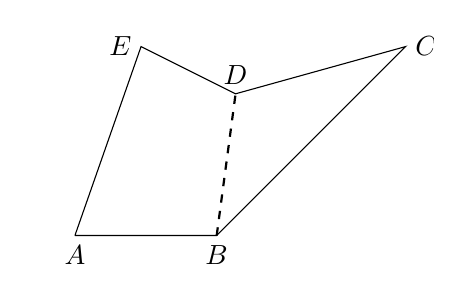
\begin{tikzpicture}[scale=1.2]
\clip (-.5,-.4) rectangle (3.8,2.2);
\draw
  (0,0) coordinate (A) -- 
  ++(1.5,0) coordinate (B) --
  ++(2,2) coordinate (C) --
  ++(-1.8,-.5) coordinate (D) --
  ++(-1,.5) coordinate (E) --
  (A);
\draw[thick,dashed] (B) -- (D);
\foreach \point/\pos in {A/below,B/below,C/right,D/above,E/left}
  \node[\pos] at (\point) {$\point$};
\vertex{B};
\vertex{D};
\end{tikzpicture}
%\includegraphics[width=\textwidth]{Fig5_11a}
    \captionof{figure}{Triangulation où une diagonale est contenue dans le polygone.}
    \label{f.contained}
     \end{minipage}
     \quad \quad %\hspace{3em}
     \begin{minipage}{0.42\textwidth}
\centering       
\begin{tikzpicture}[scale=1.2]
\clip (-.2,-.4) rectangle (3.8,2.2);
\draw
  (0,0) coordinate (A) -- 
  ++(1.5,0) coordinate (B) --
  ++(2,2) coordinate (C) --
  ++(-1.8,-.5) coordinate (D) --
  ++(-1,.5) coordinate (E) --
  ++(1.3,-1) coordinate (F) --
  (A);
\draw[thick,dashed] (B) -- (D);
\draw[very thick,dotted] (C) -- (F);
\node [draw,circle through=(F)] at (C) {};
\node[below] at (A) {$A$};
\node[below] at (B) {$B$};
\node[right] at (C) {$C$};
\node[above,yshift=2pt,xshift=-3pt] at (D) {$D$};
\node[left]  at (E) {$E$};
\node[below,yshift=-1pt,xshift=-2pt] at (F) {$F$};
\vertex{C};
\vertex{F};
\end{tikzpicture}
%\includegraphics[width=\textwidth]{Fig5_11b}
         \captionof{figure}{Triangulation où une diagonale n'est pas contenue dans le polygone.}
     \end{minipage}
\label{f.museum.concave-vertices}
\vspace{0.4cm}



Si $\overline{BD}$ n'est pas contenu dans le polygone, il doit y avoir un sommet concave $F$ qui est le plus proche de $C$ (fig.~\ref{f.museum.concave-vertices}).  $\overline{CF}$ est une diagonale qui divise le polygone en deux polygones plus petits $\overline{CFED}$ et $\overline{CFAB}$. Par l'hypothèse de récurrence, ceux-ci peuvent être triangulés et collés ensemble.\qed

\subsection*{Quelle est la surprise?}

Le théorème du musée est surprenant parce que ce qui semble être un théorème de géométrie est démontré de manière plutôt élégante par un appel au coloriage d'un graphe. 

\subsection*{Sources}

Ce chapitre se base sur \cite[chap.~39]{thebook}.